\chapter{Implementation}
\label{sec:implementation}
This section describes the implementation of the design discussed in Section~\ref{sec:design} built on top of the Wayland display server protocol. This implementation, called `Motorcar', is free and open source and available on GitHub \cite{motorcar-github}. It is intended both to demonstrate concretely that such a design is practical to implement, as well as to serve as a functional 3D windowing system and provide a modular core of that can form the basis of further research into the concept of 3D windowing systems.

\section{Wayland Protocol Extensions}

The design outlined in Section~\ref{sec:design} requires several pieces of functionality not provided by the core Wayland protocol (like synchronization of the view and projection matrices between the compositor and the clients) and functionality that is not supported by the subsystems on which Wayland in built (like the ability for the compositor to access client depth buffers), so an implementation on top of Wayland requires several extensions to the Wayland protocol to provide 3D windowing services to clients (see Section~\ref{sec:wayland-protocol} for a brief introduction to the Wayland protocol).

These protocol extensions form the basis of the 3D windowing mechanism, and are not exclusive to the compositor framework or client applications presented here. Any Wayland compositor or client could hypothetically support these extensions, allowing the basic 3D windowing mechanism to be extended to a variety of applications and integrated with client applications and tool kits as needed. The extensions are designed to be simple and flexible, so that any shortcomings of the compositor and client frameworks presented here do no limit the adoption of the 3D windowing techniques which they implement.

\subsection{Interfaces}

The protocol extensions used by Motorcar define several interfaces which the compositor uses to advertise and provide 3D windowing services to clients. Each of these interfaces is designed to provide one or more of the elements of the architecture outlined in Section~\ref{sec:design}, which is designed to require minimal extensions of existing windowing systems, so the interfaces outlined here are relatively simple.

\subsubsection{Motorcar Shell}

The first interface, `motorcar{\_}shell' represents a compositor shell that supports 3D windowing of the style discussed in this thesis, and  it has a single request, `get{\_}motorcar{\_}surface', which takes an existing Wayland surface (wl{\_}surface) as an argument and returns a new Motorcar surface which is associated with the argument Wayland surface within the compositor.  The compositor creates a single instance of this interface at startup, and clients can then use this instance to create a Motorcar surface object from the Wayland surfaces which they have already created.

\subsubsection{Motorcar Surface}

The interface `motorcar{\_}surface' represents a 3D window of the kind discussed in this thesis. It allows the client to request the type of 3D window desired (for example a cuboid or portal window) and declares events which allow the compositor to inform the client of the 3D window's bounds and transform in space and to deliver 3D input events to the client. Because the instantiation of this interface takes a Wayland surface as an argument, it allows the compositor to identify which surfaces are being used as Motorcar surfaces and composite them appropriately. When a Motorcar surface is created the compositor calculates the buffer size needed to hold the images (and depth buffers) for all of the viewpoints and resizes the surface to these dimensions.

\subsubsection{Motorcar Viewpoint}
\label{sec:viewpoint}

Perhaps the most important of the interfaces defined in the Motorcar extensions, `motorcar{\_}viewpoint' represents a virtual camera in the 3D interface space managed by the compositor (usually corresponding to one of the user's eyes), and provides the mechanisms needed to ensure that the client's 3D content is projected in a manner which allows it to be properly composited with 3D content from other clients and the compositor. This interface has no requests, only events which allow the compositor to inform clients of the parameters for the viewpoint which it represents.

The compositor creates a global instance of this interface for each viewpoint from which it is drawing the scene, allowing the client to produce correct output for each of these viewpoints. The protocol imposes no limit on the number of viewpoints or how the images produced by clients for each viewpoint are laid out within the surface, and allows viewpoints to be added or removed at runtime if necessary, leaving these things up to the compositor implementation. The example compositor presented here supports only a single user and a single stereoscopic display, and does not support hotplugging displays, so it will never instantiate any viewpoints other than the two it creates at startup (one for each of the user's eyes), but this limitation is not reflected in the protocol itself. The Motorcar viewpoint interface defines three events. 

The first two events, `view{\_}matrix' and `projection{\_}matrix', allow the compositor to update the view and projection matrices used by the client, and are sent once when the client connects, and again every time one of the matrices changes. These matrices are updated by separate events because while the view matrix changes every time the user's head moves, the projection matrix changes only when the user's head move relative to the display surface, which never happens when using an HMD (since it is strapped to their head) so the projection matrices for HMD viewpoints never changes at runtime. Some other types of immersive displays, like CAVEs, would require that the projection matrix change every time the users head moves, and while this is compatible with the protocol, it is not supported by the example compositor presented here.

The third event, called `view{\_}port', informs the client of where in the surface buffer to draw the output for the viewpoint generating the event. This allows clients to send the output of multiple viewpoints to the compositor using a single surface, which eliminates the need to synchronize updating multiple surfaces. The view port events actually defines two viewports for each viewpoint, one for the color image and one for the depth buffer, which is needed to correctly composite the 3D content from different clients (see Section~\ref{sec:depth-compositing} for details). It may seem unusual that the color and depth buffers be given different view ports in the same image, since they represent information about the same set of pixels, but this is tragically unavoidable for reasons that are somewhat complicated.

\paragraph{EGL and the Depth View Port}
\label{sec:depth-viewport}

The use of a second view port in the color buffer to transfer the contents of the depth buffer from the clients to the compositor is a significant workaround resulting from the inability of Wayland EGL to make client depth buffers accessible to the compositor. Wayland EGL allows clients to create OpenGL contexts in which the color buffer attached to the default framebuffer can be used by the compositor as a texture without ever needing to copy the memory which backs the color buffer, making it very desirable for clients which are drawing their window on the GPU (as any 3D application would certainly be doing). However, Wayland EGL does not give the compositor the same kind of access to the depth buffer attached to the default framebuffer in the client's context, which presents a significant hurdle. 
	
This is overcome by doubling the size of the color buffer attached to the client's default framebuffer, drawing into a framebuffer object whose color and depth buffers are backed by textures, and then texturing both the color buffer and the depth buffer from the framebuffer object into the color buffer attached to the default framebuffer. The compositor can then extract the original depth and color buffers from the client color buffer and write them back into the depth and color buffers of a new framebuffer, which it can then composite with the 3D scene based on the contents of the depth buffer. This introduces a significant amount of rendering overhead and is the only part of this design that cannot currently be implemented cleanly on top of Wayland. Solving this problem efficiently, by giving the compositor direct access to the depth buffer attached to the client's default framebuffer, is probably possible but would likely require modification of the implementation of Wayland EGL within Mesa. This is considered by the author to be the single most pressing area of future work on this system.

\begin{figure}[ht!]
\centering
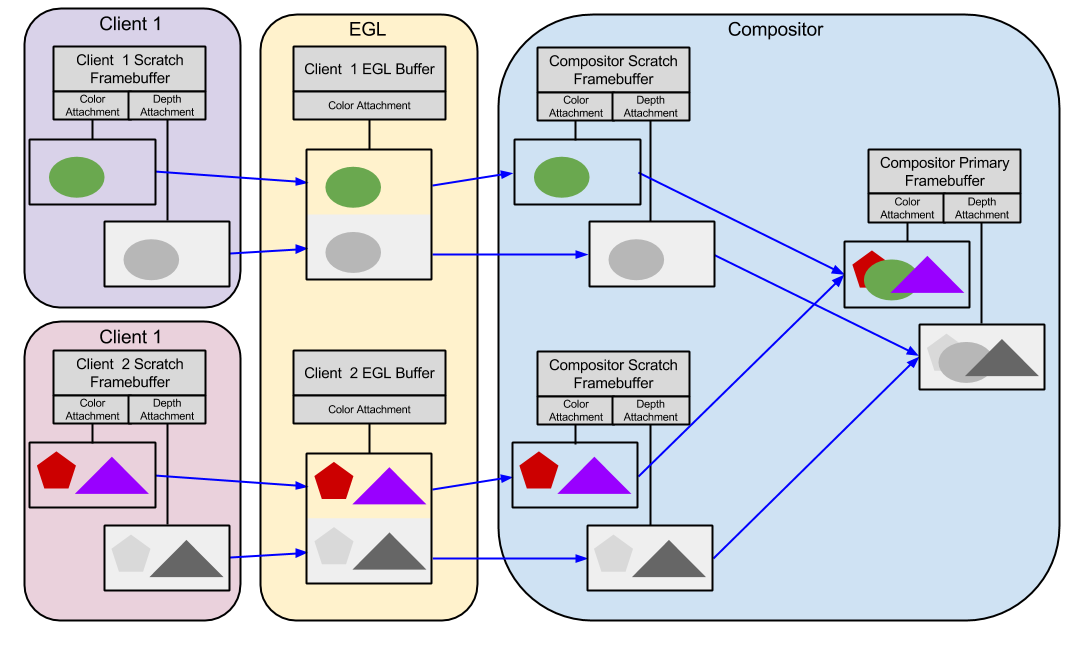
\includegraphics[width=1.0\textwidth]{images/depth-buffer-operation.png}
\caption{A high level conceptual illustration of the depth compositing process. Clients draw their depth and color images into the same, double-height color buffer, which the compositor then draws back into normal sized depth and color buffers, and then composites with other 3D clients using the traditional depth test. Lighter color in the depth images indicates that those pixels are further away.}
\end{figure}

The process of encoding the depth buffer contents in the color buffer is further complicated by the differences between the format of the depth buffer and color buffer. The example compositor uses a color format that allocates eight bits for for each of four color channels (red, green, blue, and alpha, which is used here for transparency) and a 16 bit integer depth format. In order to transfer the depth information without loss of precision the system presented here samples the depth buffer on the client side as a 32 bit float, then uses a technique taken from \cite{pack-float-rgba} to pack this float into a four-vector which is then written into the color buffer and unpacked back into the 32 bit float on the compositor side (using the reverse technique from \cite{pack-float-rgba}) and written back into the depth buffer. 

\subsection{Current Protocol Limitations}
In its current state the Motorcar protocol extensions has very basic support for 3D input events. The only implemented input events are essentially the 3D equivalent of mouse events, such as button pressed attached to a six degree of freedom (6DOF) transform, or changes in this 6DOF transform. These kinds of events form a good extension of mouse events to 3D, and map well onto the input device used in this implementation (the Razer Hydra 6DOF handset), but they certainly do not encompass all possible 3D input. Other broad classes of input events include skeleton tracking and gesture events, and these types of events could certainly be delivered over additional Wayland protocol extensions. However, an abstraction layer for these types of events would require the development and integration of substantial systems which are well outside the scope of this thesis, so they are excluded from this version of the Motorcar protocol extensions.

\section{Client Operation}

This section describes the operation of 3D clients using the Motorcar protocol extensions, and most of this is firmly grounded in the way that the sample 3D clients provided by Motorocar operate. The operation of 2D clients is not discussed in detail here because it is literally identical to standard Wayland client operation, which is a key feature of this system because it allows unmodified 2D clients to window into the 3D interface space without even being aware of its three dimensional nature. The example Motorcar client code is derived from the weston-simple-egl client distributed with Weston (the Wayland reference compositor), but adapted from C to C++ and repackaged as an interface which can be implemented by individual clients with minimal effort.

When the client connects to the compositor it receives creation events for all of the global objects instantiated by the compositor, including the Motorcar shell and all of the Motorcar viewpoints. The client can use the Motorcar shell to create a Motorcar surface from any Wayland surfaces it create, which tells the compositor to handle that surface as a Motorcar surface (since these are composited differently than normal surfaces) and allows the compositor to send 3D input events to that client, which the client can listen for if it chooses. 

The client binds each viewpoint and creates a data structure to represent it internally, which it then attaches to the event listener for that viewpoint. The compositor responds to the binding process by sending the client the current state of the viewpoint (its view and projection matrices and its view port) to the client, which the client then stores in the data structure associated with that viewpoint.

Every time the client gets the frame callback indicating that it should draw a new frame, it iterates over all of the viewpoints and draws it's scene however it likes with the view and projection matrices from that view point into the viewpoint's color view port, then copies the depth buffer for that viewpoint into the viewpoint's depth view port. Once this has been done for each of the viewpoints the client calls eglSwapBuffers, which swaps the surfaces front and back buffers and informs the compositor that surface is ready to be updated.

\section{Compositor Operation}

This section describes the operation of the Motorcar compositor implemented for this thesis. There are other ways that a Motorcar protocol compliant compositor could function, but enumerating all of these designs is an intractably large task and likely would not be useful anyway, so instead this section focuses on the concrete aspects of the design that was implemented and is known to work. The operation of the compositor is complex, and an exhaustive discussion of this software that implements it would be obscenely long, so the discussion here is limited to the components of the compositor which are relevant to the mechanism by which is provides 3D windowing services to clients. Users seeking a more comprehensive understanding of the structure of this software are directed to the documentation in the GitHub repository \cite{motorcar-github}.

\subsection{The Motorcar Compositor Framework}

This thesis presents a modular C++ framework for Motorcar compositors designed to be extremely flexible in the way that 3D windowing services are provided to clients. The main function of a compositor built with this framework essentially just initializes components which implement interfaces defined in the framework and attaches them to one another over these interfaces. This allows components which do not meet the needs of a particular compositor to be replaced by ones that do without needing to rebuild the compositor from scratch, and it allows new components to be defined and attached in natural ways. Examples of modules which would likely be replaced are device specific classes (which implement device interfaces for things like 3D pointing devices or head mounted displays on top of device specific API's) and the window manager (which controls how input events are directed to clients and how surfaces are laid out in 3D when they are mapped).

\subsubsection{The QtWayland Motorcar Compositor}

The Motorcar compositor implemented for this thesis uses several core components built on top of the QtWayland Compositor API. QtWayland is a module in the Qt toolkit which provides a Wayland backend for graphical Qt applications, as well as providing a simple framework for building Wayland compositors on top of Qt. All of the QtWayland dependent functionality in this compositor is isolated within a small set of classes which hide the QtWayland functionality behind interfaces defined in the Motorcar framework, which could hypothetically allow it to be separated and allow Motorcar compositors to be built without a Qt dependency, though this is not necessarily desirable.  

QtWayland abstracts almost all of the interaction with the Wayland protocol itself (with the exception of interactions with the Motorcar protocol extensions) behind a set of C++ classes which form the QtWayland Compositor interface, and most of these classes interact with the Motorcar compositor framework through thin wrapper classes which exist primarily to isolate the Qt dependency. It handles almost all of the behaviour needed to correctly interact with 2D clients, allowing the Motorcar compositor framework to focus on embedding the 2D clients' surfaces in the 3D space and correctly sending these surfaces input events in their local coordinate system. Additionally, Qt provides a platform independent OpenGL context, which allows QtWayland compositors to run within other Wayland Compositors, within an X environment, or even directly on top of the user interface hardware abstractions in the Linux kernel.

\subsubsection{The Compositor Scene Graph}



The compositor maintains an internal scene graph which contains all spatial elements in the 3D interface space. This includes surfaces (for both 2D and 3D windows), viewpoints, displays, input devices, models of the user skeleton, and any graphical interface elements drawn by the compositor (for example window decorations or docks). All scene graph classes inherit from a root class called SceneGraphNode, which provides spatial relationship primitives as well as defining a doubly linked tree structure between nodes (which forms the actual graph of the scene) and provides mechanisms for traversing this tree. 

All scene graph nodes have a single parent and a list of children, and these are made accessible so that other parts of the compositor can manipulate the scene graph as they see fit, and these two members form the core of the functionality that the SceneGraphNode class provides. The scene graph is rooted in an instance of a special scene graph class called Scene (which is unique in being allowed to have a null parent), and this forms the primary interface between scene graph classes (which can always access the scene root by traversing up the scene graph) and classes like the window manager, motorcar shell, and display server modules (which typically are constructed with a pointer to the scene on which they operate).

\begin{figure}[ht!]
\centering
\includegraphics[width=1.0\textwidth]{images/scene-graph-classes.png}
\caption{The inheritance graph for the classes composing the scene graph. Note the division between virtual nodes (which can be children of any other node) and physical nodes (which can only be children of other physical nodes) to reflect the impossibility of a physical object being attached to a virtual one.}
\label{fig:scenegraph-classes}
\end{figure}

\paragraph{Traversing the Scene Graph}

The scene graph is designed to be traversed several times per frame, and the SceneGraphNode class provides virtual methods which allow implementing classes respond to each of these traversals appropriately without needing to implement the traversal logic themselves. The first traversal, invoked immediately prior to sending the current viewpoints to the clients and requesting new data from them, is intended to allow implementing classes to do per-frame work prior to rendering (for example animation updates or event generation by devices) and is handled by overriding SceneGraphNode::handleFrameBegin(). The second traversal, invoked once per display per frame, is intended to allow implementing classes to render their content to the display and is what drives surface classes to perform the compositing operations discusses in Section~\ref{sec:3d-compositing}. This traversal can be handled directly by overriding SceneGraphNode::handleFrameDraw(), but most classes that respond to this traversal should inherit Drawable and override Drawable::draw() instead. The third and final traversal, invoked every frame after drawing is completed and handled by overriding SceneGraphNode::handleFrameEnd(), in intended to allow any implementing classes to clean up any resources which were created during the first traversal that will not be needed in the next frame.

\subsection{Frame Timing and Latency}

This design requires that the compositor send new view matrices to its 3D clients every frame, wait for them to draw new images, and then composite these images and send them to the display before the next frame starts, so getting the timing correct is a little bit tricky and there are several possible approaches with merit. 

The approach taken in this implementation is to draw the scene graph (the handleFrameDraw traversal) with the current data at the beginning of the frame, clean up the frame (the handleFrameEnd traversal), update the scene graph state (the handleFrameBegin traversal), then send the new matrices to the clients followed by the frame callbacks that tell them to draw a new frame, then wait until the next vSync event (indicating the display is done drawing) to swap the compositor buffers and restart the process. This approach favours using old client output over dropping frames in the compositor because it gives clients only the time remaining in the frame after compositing completes to update their content before the compositor simply uses the output it already has in memory. This ensures that no single client can reduce the compositor frame rate, but it also means that 3D clients can get out of sync with the compositor, which would break the illusion of a unified 3D interface space (because out-of-sync clients would be drawn from a viewpoint that has since changed). Additionally, this means that the time it takes a movement of the user's head to affect the image drawn appropriately (referred to as `motion-to-photon latency') would include an entire extra frame's worth of time, which is undesirable in certain applications.

An alternative approach would be to update the scene graph, send the new matrices and frame callbacks to the 3D clients, wait until all of the 3D clients have finished drawing, and only then draw the scene and clean up. This approach would minimize the motion-to-photon latency but, because it requires that the compositor wait for the clients to finish drawing, it could allow a single slow client to cause the compositor to drop frames. This approach may be more suitable for applications like immersive virtual reality video games, where only a single latency-sensitive application needs compositing, and it is probably not the most general purpose solution. As discussed in Section~\ref{sec:vr-mode}, this timing mode could potentially be toggled from the client based on its application profile, though such functionality is not yet implemented in the system presented here.

\subsection{Three Dimensional Compositing}
\label{sec:3d-compositing}

The core functionality of a Motorcar compositor is its ability to combine interfaces from 2D and 3D applications in a unified 3D interface space. The compositing portion of this requires that the compositor be able to draw 2D windows on planes embedded in the 3D space and be able to composite the output from 3D applications with these planes as well as with the output of other 3D applications. The first requirement is fairly straightforward (especially with the use of QtWayland), essentially boiling down to projecting and texturing quads with OpenGL, so we do not bother to discuss it in detail here. The second requirement is met with a fairly complex mechanism that forms one of the core contributions of this thesis, and this mechanism is the focus of the rest of this section.

When clients create a Motorcar surface, the scene graph node representing the surface (of class WaylandSurfaceNode) is replaced by a new node with an inheriting type (class DepthCompositedSurfaceNode)  that defines the correct compositing behaviour for Motorcar surfaces. The DepthCompositedSurfaceNode class performs the compositing operations needed to make the contents of its surface appear three dimensional to the user.

\subsubsection{Clipping and Depth Compositing}
\label{sec:clipping-impl}

The clipping process varies slightly depending on the type of window being clipped, but for the most part the process is identical. The term `near clipping surface' is used here to describe the surface which the everything in the window must be in front of, the term `far clipping surface' is used to describe the surface which everything in the window must be drawn in front of, and `full clipping surface' is used to describe the union of these two. For a cuboid window the near clipping surface is the three faces of the cuboid facing toward the viewpoint (the first three faces where the dot product of the face normal and the view vector is less than or equal to zero) and the far clipping surface is the other three faces of the cuboid. For portal type windows the near clipping surface is the window opening and the far clipping surface doesn't exist. The depth compositing and clipping process uses a scratch framebuffer with the same dimensions as the compositor buffer and the process described here operates once per viewpoint.

This scratch framebuffer is first cleared (zeroing the red, green, blue, and alpha values), and the full clipping surface of of the window is written into the stencil buffer (such that only pixels within the projection of the clipping surface can be drawn to) with the color and depth buffers disabled. This prevents the client from drawing any fragments which can not possibly be valid because they are outside the projection of its window bounds, and substantially reduces the overhead of copying pixels because pixels disabled by the stencil buffer will simply be ignored. The next step is to draw the client buffer into the color and depth buffers of the scratch framebuffer using the late depth test (the depth image is extracted from the client color buffer, due to the problem described in Section~\ref{sec:depth-viewport}). This draws only those pixels which are closer than the far clipping surface, since those which are further away will fail the depth test. This draw is also where the stencil buffer drops all fragments outside the projection of the window. Next, the near clipping surface is drawn into the color and depth buffer with a completely zero color (including alpha), blending disabled, and the depth test reversed (so that fragments with greater depth pass the depth test). This replaces any fragments from the client image which are closer than the near clipping surface with the scratch framebuffer's clear color, effectively eliminating them. Finally, the contents of the scratch framebuffer (both depth and color) are drawn into the compositor framebuffer using the late depth test and a special fragment shader which drops fragments whose alpha values are zero, which prevents the depth of the clipping surfaces from polluting the compositor depth buffer. 

This process ensures both that any fragments in the client buffer which lie outside the window bounds are discarded and that any fragments inside the window bounds are composited properly.


\section{Test Hardware Configuration}

This compositor was developed using an Oculus Rift DK1 virtual reality headset and a Sixense Razer Hydra six degree of freedom magnetic tracking handset system. The Rift provides only head orientation tracking, which does not allow proper motion parallax to be simulated (see Section~\ref{sec:motion-parallax-and-stereopsis} for details. Fortunately, the Hydra system comes with two handsets, which allows one to be used to track the head's position (by attaching it to the back of the Rift headset), while the other is used as an input device. This setup can be seen in Figure~\ref{fig:hardware-setup}.

\begin{figure}[ht!]
\centering
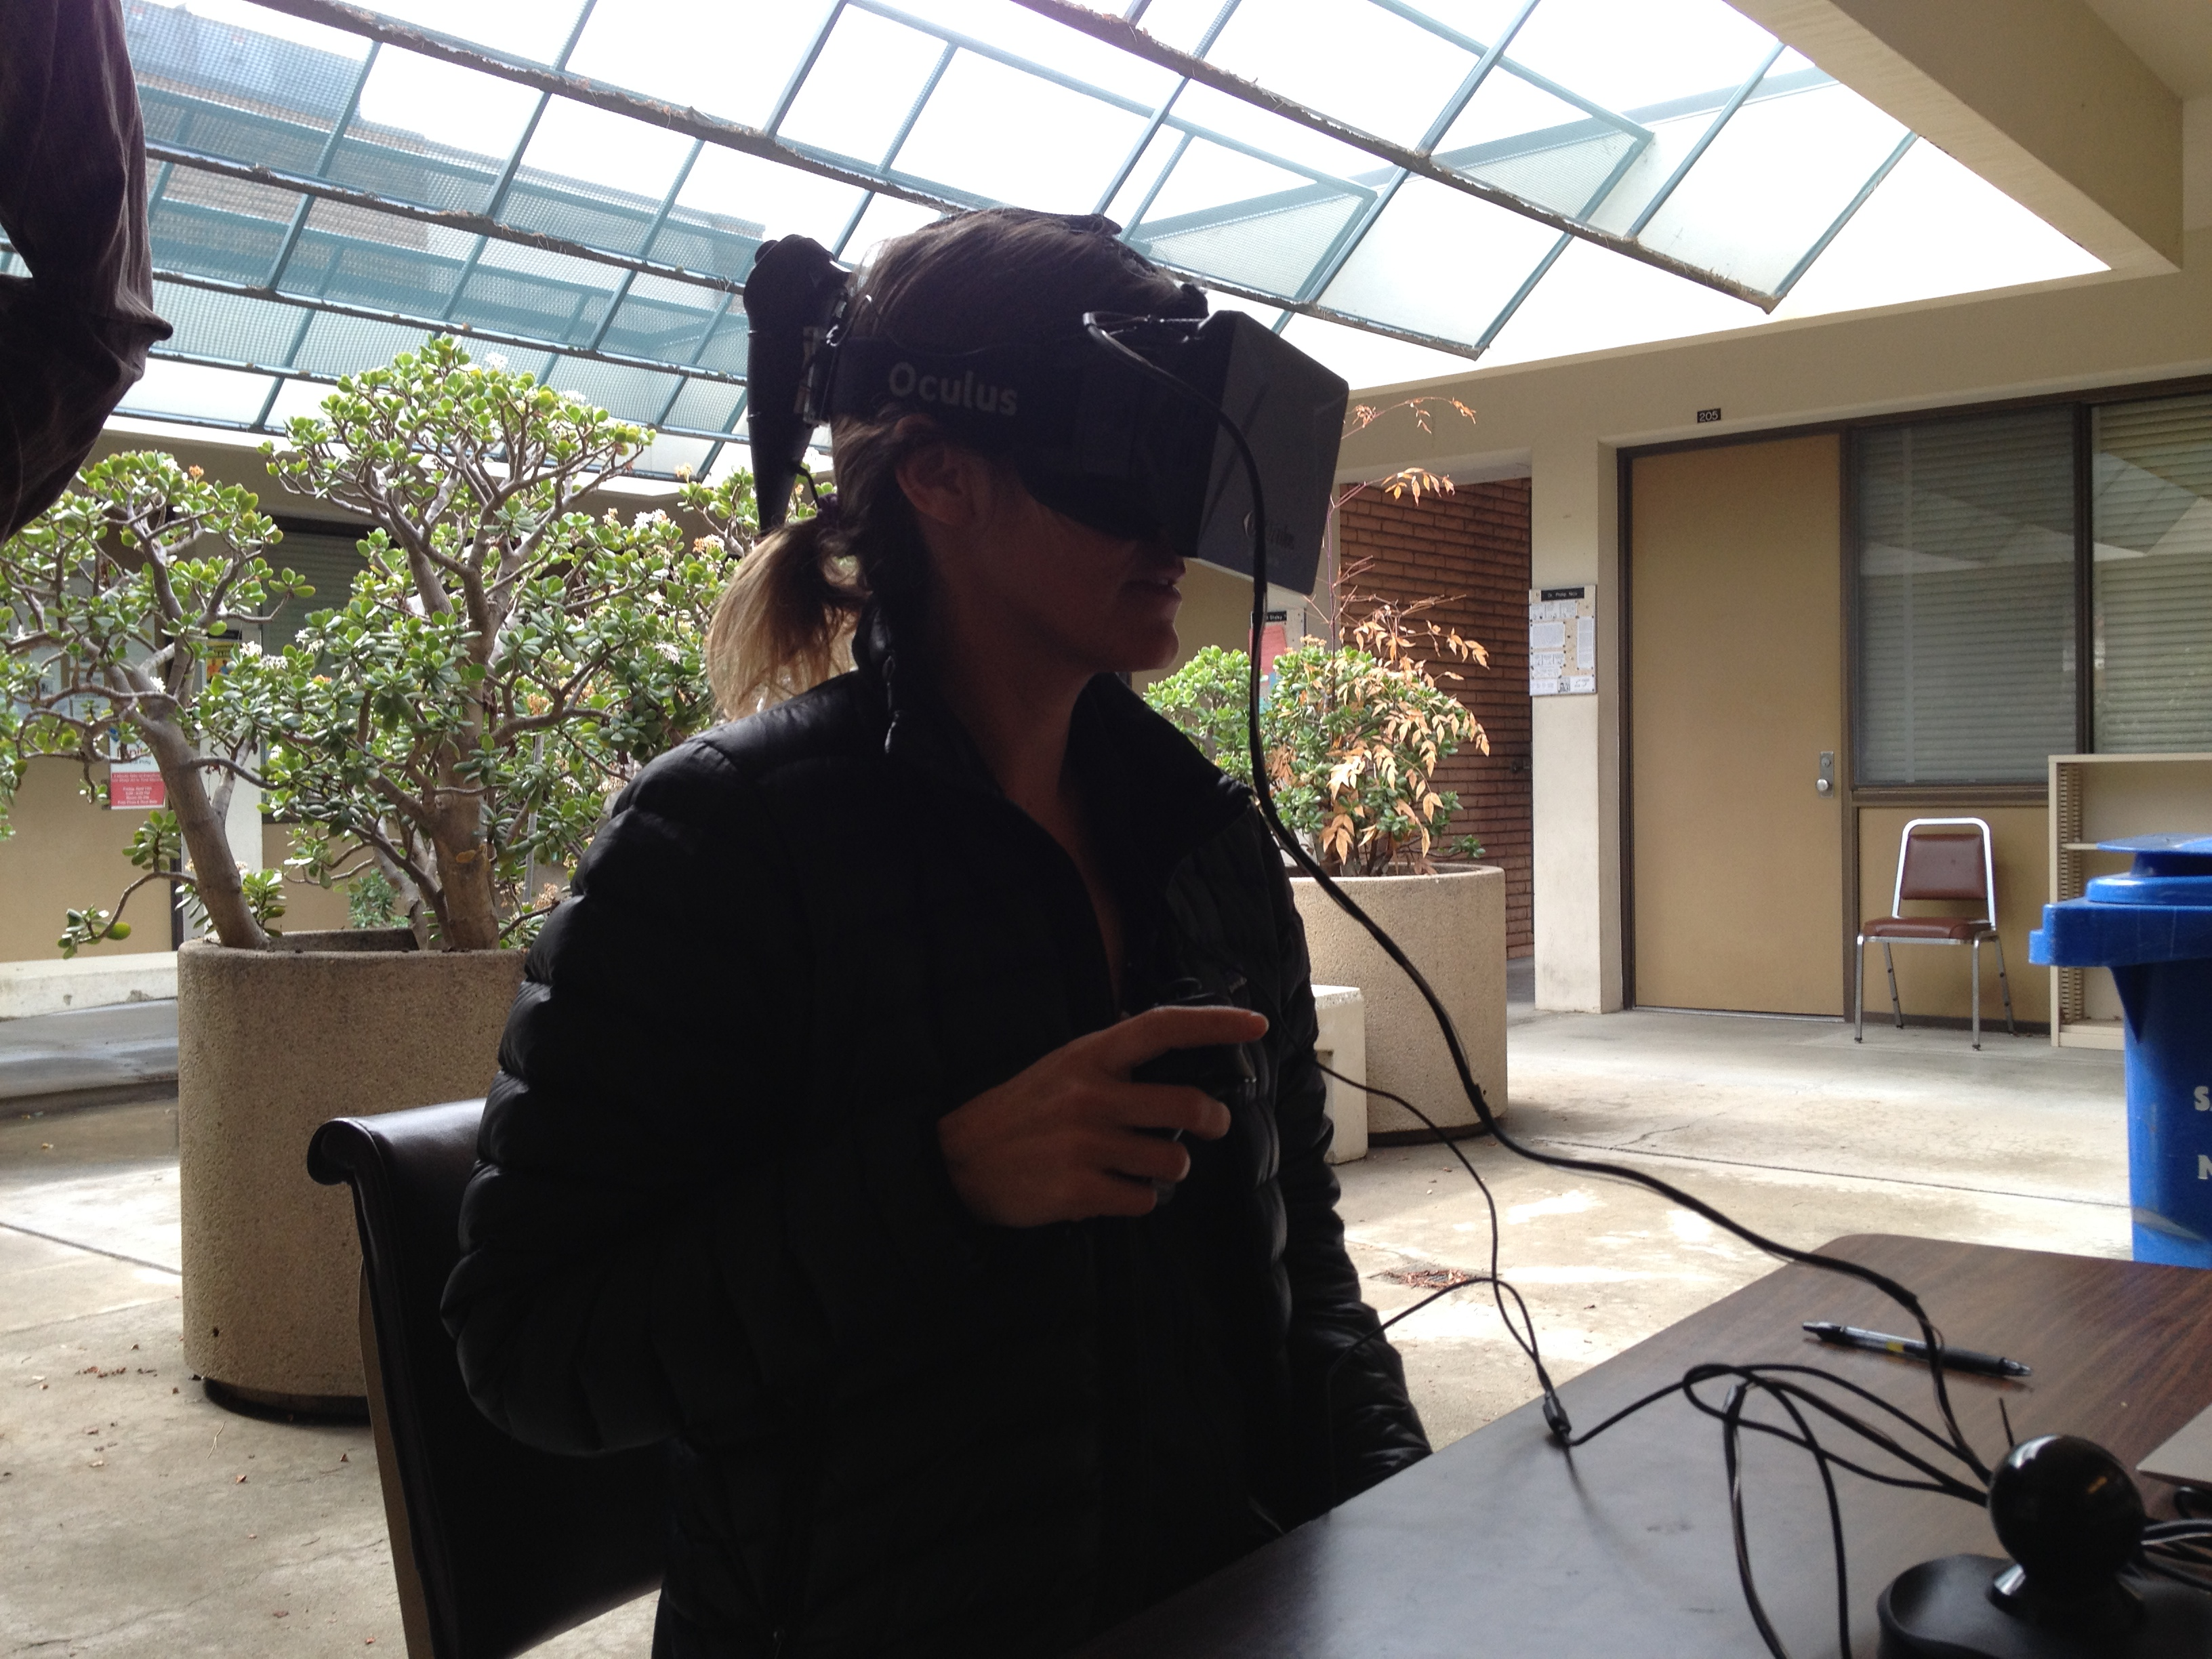
\includegraphics[width=1.0\textwidth]{images/hardware-setup.jpg}
\caption{A test subject wearing the hardware system on which this implementation was developed. Notice that one Hydra handset is held in her right hand and being used for 3D input, while the other is attached to the Rift headset and used for traking the position of the head.}
\label{fig:hardware-setup}
\end{figure}

The Oculus Rift requires a image space barrel distortion of the rendered stereo image to correct for a pincushion distortion introduced by the optics in the headset. This is performed as a final step immediately before the compositor sends the final image to the display. Clients need not even be aware of this step, which is yet another advantage of using the windowing approach described here.











